\chapter{CONSTRUCTING THE ABSTRACT SYNTAX TREE}

This section describes in detail every syntactical construct of \emph{Scandal}. For each of them there is a corresponding \emhp{Java} class with the same name. What follows is restricted to stating their abstract syntax definitions, and how they are implemented in the parser from their corresponding concrete rules. The particularities of type-checking and generating bytecode will be discussed in the next chapters. Constructs that either have trivial implementations, or whose implementations are, \emph{mutatis mutandis}, identical to other constructs are omitted, in which case only a representative is described. In the discussion below, productions begin with an upper-case letter to denote they are abstract counterparts to concrete rules with the same name beginning with a lower-case letter. Whereas all-capitalized rules referred to terminal symbols in the concrete syntax, here they refer to enumeration cases. Abstract all-capitalized rules that refer to types are cases of the \il{Types} enumeration, and all other abstract all-capitalized rules are cases of the \il{Token} enumeration.

\section{The \il{Program} Class}

The root of a \emph{Scandal} AST is always a program, which contains declarations and statements as sub-nodes. Declarations in the AST are instances of \il{Declaration}, an abstract class that has two subclasses: \il{AssignmentDeclaration}, and \il{ParamDeclaration}. The former unfolds into two subclasses, \il{FieldDeclaration}, and \il{LambdaLitDeclaration}, while the latter has no subclasses. The primary difference between the two subclasses of \il{Declaration} is that parameter declarations define a type and a name without binding any value to that name at the time of declaration, while assignment declarations require that some expression be bound to the name at the moment the variable is declared. An instance of \il{Program} can contain any number of assignment declarations, field declarations, or lambda literal declarations, in any order, while parameter declarations only exist in the context of lambda literals. Statements are the other type of top-level construct in \emph{Scandal}, and all statements in the AST are subclasses of \il{Statement}, which is also abstract. There are nine different types of statements providing various functionalities to the language. Statements may be regarded as void-returning functions, and represent the imperative side of \emph{Scandal}. Below are the abstract syntax rules for top-level constructs.

\begin{itemize}
	\item Program := (AssignmentDeclaration $|$ FieldDeclaration)$^*$
	\item Program := (LambdaLitDeclaration $|$ Statement)$^*$
\end{itemize}

The parsing routine that constructs an instance of \il{Program} is very simple, and does so by checking whether the next token in the array of tokens produced by the scanner is in the FIRST set of a declaration. If so, it attempts to construct an instance of \il{AssignmentDeclaration}, consuming in the process all the tokens therein. If not, it attempts to construct a subclass of the abstract type \il{Statement}. That is done much that same way, by looking at the FIRST set of a statement. Listing \ref{alg:program} shows how a \il{Program} node is instantiated in the AST.

\begin{lstlisting}[language=Java,caption={Parsing topmost-level constructs in \emph{Scandal}.},label={alg:program}]
public Program parse() throws Exception {
	Token firstToken = token;
	ArrayList<Node> nodes = new ArrayList<>();
	while (token.kind != EOF) {
		if (token.isDeclaration()) nodes.add(assignmentDeclaration());
		else nodes.add(statement());
	}
	matchEOF();
	return new Program(firstToken, nodes);
}
\end{lstlisting}

\begin{enumerate}
	\addtocounter{enumi}{1}
	\item Line 2 stores a reference to the first token, since this token will be consumed during the instantiation of sub-nodes, but is needed as an argument to the constructor of \il{Program} in line 9.
	\item An instance of \il{Program} holds an array of nodes. These nodes, however, must be either a subclass of \il{AssignmentDeclaration}, or a subclass of the abstract class \il{Statement}. Nodes are added in the exact order in which they appear in the \emph{Scandal} program, regardless whether they are declarations or statements.
	\addtocounter{enumi}{1}
	\item Line 5 checks whether the next unconsumed token is in the FIRST set of a declaration. If so, further parsing is delegated to the \il{assignmentDeclaration} routine. If not, the only other legal option is that the next token initiates a statement, and parsing thereof is delegated to the \il{statement} routine in line 6.
	\addtocounter{enumi}{2}
	\item An end-of-file token was included in the scanning process for convenience, and \il{parse} makes use of it by checking the next available token against the \texttt{EOF} kind. As soon as it finds it, it knows it has reached the end of the token array, and can thus stop looking for declarations and statements. If a particular token was expected, but \texttt{EOF} appeared prematurely, \il{matchEOF} throws an error.
\end{enumerate}

\section{Subclasses of \il{Declaration}}

The class \il{Declaration} is an abstract type that extends \il{Node} by adding three instance variables, namely a \il{Token} to hold the name being declared, an integer to hold its slot number, and a boolean property to distinguish whether this is a field or not. Slot numbers are not necessary for fields, hence are only used in the context of the \emph{Java} class' \il{run} method. \il{Declaration} branches out into two non-abstract subclasses, \il{ParamDeclaration} and \il{AssignmentDeclaration}. The latter has itself two other subclasses, \il{FieldDeclaration} and \il{LambdaLitDeclaration}. As discussed above, the difference is that \il{ParamDeclaration} only occurs inside a \il{LambdaLitDeclaration}; \il{FieldDeclaration} and \il{LambdaLitDeclaration} only occur at the outermost scope; and \il{AssignmentDeclaration} occurs anywhere. Below are the abstract syntax rules for declarations. In these abstract rules, an \texttt{IDENT} has a different meaning than its concrete counterpart. Here it is an instance of \il{Token}, rather than a character string. Similarly, types are converted after parsed into enumeration cases of \il{Types}, according to the keyword at hand.

\begin{itemize}
	\item AssignmentDeclaration := Types Token.\texttt{IDENT} Expression
	\item FieldDeclaration := Types Token.\texttt{IDENT} Expression
	\item LambdaLitDeclaration := Types.\texttt{LAMBDA} Token.\texttt{IDENT} LambdaLitExpression
	\item LambdaLitDeclaration := Types.\texttt{LAMBDA} Token.\texttt{IDENT} LambdaLitBlock
	\item ParamDeclaration := Types Token.\texttt{IDENT}
	\item Types := \texttt{INT} $|$ \texttt{FLOAT} $|$ \texttt{BOOL} $|$ \texttt{STRING} $|$ \texttt{ARRAY} $|$ \texttt{LAMBDA}
\end{itemize}

As shown in line 5 of Listing \ref{alg:program}, declarations are parsed by looking at the very first token at hand, since FIRST(declaration) = type $\cup$ \texttt{KW\_FIELD}. Listing \ref{alg:assign} demonstrates how the various types of top-level declarations are constructed in the parser by the \il{assignmentDeclaration} routine. The sections below describe how each type of declaration differs from \il{Declaration} in their \emph{Java} implementations.

\begin{lstlisting}[language=Java,caption={Parsing Top-Level Declarations.},label={alg:assign}]
public AssignmentDeclaration assignmentDeclaration() throws Exception {
	boolean isField = token.kind == KW_FIELD;
	if (isField) consume();
	Token firstToken = consume();
	Token identToken = match(IDENT);
	match(ASSIGN);
	Expression e = expression();
	if (e instanceof LambdaLitExpression)
		return new LambdaLitDeclaration(firstToken, identToken, e);
	if (isField) return new FieldDeclaration(firstToken, identToken, e);
	return new AssignmentDeclaration(firstToken, identToken, e);
}
\end{lstlisting}

\begin{enumerate}
	\addtocounter{enumi}{1}
	\item Observing that \il{FieldDeclaration} is the only subclass of \il{Declaration} that may possibly make use of a \il{field} flag, \il{assignmentDeclaration} begins parsing by first checking whether the first token of a declaration is indeed a \il{field} flag, setting a local boolean property accordingly, and consuming the \texttt{KW\_FIELD} token in line 3.
	\addtocounter{enumi}{1}
	\item Lines 4 to 7 store the type (first) and identifier tokens, consume the equals sign, and delegate the expression's parsing to the \il{expression} routine. Unassigned declarations will fail the \il{match(ASSIGN)} call in line 6, and will cause a compilation error. Based on the type of expression received, a corresponding subclass of \il{AssignmentDeclaration} is constructed.
	\addtocounter{enumi}{3}
	\item Line 8 checks if the parsed expression is an instance of \il{LambdaLitExpression}, in which case line 9 constructs a \il{LambdaLitDeclaration}. Even though lambda literal declarations are always fields in the \emph{Java} class, the \il{field} flag is not necessary, but \emph{can} be used without errors, since all that determines an instance of \il{LambdaLitDeclaration} is that the expression it contains is a subclass of \il{LambdaLitExpression}.
	\item If not a lambda literal, then line 10 checks if a field flag was given, constructing a \il{FieldDeclaration} if so. If control reaches line 11, then a generic \il{AssignmentDeclaration} is returned instead.
\end{enumerate}

\subsection{The \il{AssignmentDeclaration} Class}

Assignment declarations are the most general an common type of top-level declaration in \emph{Scandal}. They correspond to all variable declarations that are not \emph{special}, neither in the sense of featuring an expression that contains a method body, nor in the sense of being global to a \emph{Scandal} program. In other words, they live inside the \emhp{Java} class' \il{run} method, as well as inside a lambda's body. Since the \il{isField} property is false by default, an instance of \il{AssignmentDeclaration} is constructed by passing a type token and an identifier token to the superclass, then storing an \il{expression} property, the latter being what differentiates assignment declarations from the abstract type \il{Declaration}.

\subsection{The \il{LambdaLitDeclaration} Class}

The \il{LambdaLitDeclaration} class is a particular case of \il{AssignmentDeclaration} where the stored expression property is of type \il{LambdaLitExpression}. By defining a new type, instances of lambda literals are more easily separated from other nodes inside a \il{Program}. As shall be seen in the the chapter on type-checking, having a specific type for lambda declarations is also invaluable when the underlying implementation of a lambda is obscured by partial applications and compositions, in which case an entire chain of bindings may need to be unraveled until a name that is bound to an expression of type \il{LambdaLitDeclaration} is found. A lambda literal declaration is constructed by taking a \il{LambdaLitExpression}, and passing it to the constructor of the superclass. It follows the superclass' \il{expression} property is just a reference to this lambda literal expression property, which is called \il{lambda}. Naturally, every \il{LambdaLiteralExpression} inherits from \il{Expression}. At the time a lambda literal declaration is constructed, the \il{isField} boolean property is also immediately set to true.

\subsection{The \il{FieldDeclaration} Class}

Field declarations are possibly the simplest type of declaration in the AST. They mostly exist for convenience, in order not to clutter its superclass \il{AssignmentDeclaration}, which has a somewhat more involved implementation. Field declarations are constructed by calling the superclass' constructor with exactly the same arguments that were given to the constructor of \il{FieldDeclaration}, and by setting the \il{isField} boolean property to true.

\subsection{The \il{ParamDeclaration} Class}

\il{ParamDeclaration} is basically an unchanged implementation of the abstract type \il{Declaration}. It adds no properties to it, thus consisting of basically a type \il{Token} and an identifier \il{Token}. Since it is not abstract, it must override \il{decorate} and \il{generate}, the two abstract methods in \il{Node} that provide functionality to all nodes in the AST. Parsing a parameter declaration is absolutely straightforward, and done in the context of a \il{LambdaLitExpression}. The parsing routine for a parameter declaration simply stores and consumes the type and identifier tokens, then uses those to instantiate a \il{ParameterDeclaration} class.

\section{Subclasses of \il{Statement}}

Statements and declarations are the only types of top-level constructs that \emph{Scandal} supports. Statements can occur freely inside any scope, and are essential for the language in that they provide much of its core functionality. As seen above in Listing \ref{alg:program}, parsing statements is accomplished the same way declarations are, by looking at the FIRST set of each statement. Except for assignment statements, whose first token is an identifier, every statement in the language begins with a keyword. The \il{statement} routine in the parser contains a \il{switch} with cases for \texttt{IDENT} and every statement keyword, and defaults to throwing an error if the first token given does not match any of these kinds. Depending on the keyword, the parser instantiates one of the particular subclasses of \il{Statement}. Below are the abstract syntax rules for statements.

\begin{itemize}
	\item Statement := ImportStatement $|$ IfStatement $|$ WhileStatement
	\item Statement := AssignmentStatement $|$ IndexedAssignmentStatement
	\item Statement := PrintStatement $|$ PlotStatement $|$ PlayStatement $|$ WriteStatement
	\item ImportStatement := Expression
	\item IfStatement := Expression Block
	\item WhileStatement := Expression Block
	\item Block := (AssignmentDeclaration $|$ Statement)$^*$
	\item AssignmentStatement := Token.\texttt{IDENT} Expression
	\item IndexedAssignmentStatement := Token.\texttt{IDENT} Expression\_0 Expression\_1
	\item PrintStatement := Expression
	\item PlotStatement := Expression\_0 Expression\_1 Expression\_2
	\item PlayStatement := Expression\_0 Expression\_1
	\item WriteStatement := Expression\_0 Expression\_1 Expression\_2
\end{itemize}

There are four varieties of statements in \emph{Scandal}: compiler statements, control statements, assignment statements, and framework statements. Compiler statements are restricted to import statements at the moment. Control statements are if and while-loops. Assignments simply bind a new expression to a previously declared variable. Framework statements define the specific domain of the language, and consist of four hooks to the \emph{Java} audio engine, namely routines to print to the console, playback a buffer of audio data with a given number of channels, plot a decimated array of floats, and write a \emph{.wav} file to disk. Framework statements may be regarded as \il{void} methods, since they never return anything. There exist other hard-wired routines in \emph{Scandal} that do return some expression, and are thus treated as such and discussed later. The \il{Statement} class extends \il{Node} but is itself abstract. It is constructed with an instance of \il{Token}, that in turn is used to call the constructor of its superclass, and an instance of \il{Expression}, which is stored. Every statement in \emph{Scandal} contains at least one expression, but their purposes vary according to the statement type. In converting from concrete rules into abstract ones, assignments, parenthesis, commas, and braces are all discarded, and most statements are in essence a collection of expressions. The exceptions are conditional statements, which also contain blocks.

\subsection{The \il{ImportStatement} Class}

Import statements are the simplest type of statement in \emhp{Scandal}. The \il{ImportStatement} class extends \il{Statement}, but adds no properties to it. Each import statement accepts a single expression of type \il{string} containing a path in the file system to a \emph{.scandal} file. Import statements are used by the compiler as described in Listing \ref{alg:link}, wherein all import statements in a chain of linked programs form a DAG. A depth-first search of the DAG pre-compiles every program in it, that is, creates an AST for them without decorating or generating bytecode. Paths are then extracted from import statements in order, which effectively creates a reverse topological sorting of the graph. If the chain of imported programs contains a cycle, then execution will fail at runtime.

\subsection{Control Statements}

Both control statements in \emph{Scandal} extend \il{Node} by including a \il{block} property. The basic functionality of a block is to introduce a new scope of declarations and statements. These are executed one or more times, depending on the type of conditional, should the test following the conditional keyword succeed. The \il{Block} class, in turn, extends \il{Node} by including an array of nodes, similarly to the \il{Program} class. Like the latter, these nodes may be assignment declarations or statements. Parsing blocks is very similar to parsing top-level constructs. The basic difference is that a block is surrounded by braces, thus parsing begins by consuming the left brace. It then looks for declarations or statements until a right brace is found, throwing an error if not. The parser routines that create these declarations and statements are exactly the same that create top-level constructs. Conditional statements are parsed by consuming the first token, asking the \il{expression} method in the parser for an expression, and finally asking the \il{block} method for a block.

\subsection{Assignment Statements}

The \il{AssignmentStatement} class extends \il{Statement} by including a \il{declaration} property and, naturally, overriding both \il{decorate} and \il{generate} methods. \il{AssignmentStatement} has a subclass that specializes in assigning float values to an array at particular indices. \il{IndexedAssignmentStatement} extends \il{AssignmentStatement} by including an expression property that holds the index at which the array is to be assigned. Indexed assignment statements are parsed alongside its superclass by observing that PREDICT(indexedAssignmentStatement) = PREDICT(assignmentStatement). Differentiating between indexed and non-indexed assignments is accomplished by consuming the identifier, then checking if the next token is a left bracket. An instance of \il{IndexedAssignmentStatement} is constructed by passing along the \il{declaration} and \il{expression} properties to the constructor of the superclass, then storing the \il{index} property.

\subsection{Framework Statements}

Print statements provide the functionality of printing to the IDE's console the value of strings, floats, integers, and booleans. They extend \il{Statement} only by implementing both \il{decorate} and \il{generate} methods. As with import statements, print statements take a single expression as input, hence a print statement is needed for each expression posted to the console. Print statements are parsed by consuming and converting the \il{print} keyword into a \il{Token}, then asking the parser's \il{expression} routine for a subclass of \il{Expression}. The token and expression are used to instantiate a \il{PrintStatement} class, whose constructor simply calls the superclass' constructor.

The \il{PlotStatement} class extends \il{Statement} by including two more expressions. The three expression properties are namely a string to display a title for the plot, an array of points to be plotted, and an integer defining the number of points to be plotted. Since arrays of audio samples can be quite long, the last parameter is used to decimate an array if it is longer than the specified number of points. If it is shorter, the \il{PlotTab} class in the IDE will oversample the array to have the specified length. Plot statements are parsed by consuming the keyword and a left parenthesis, then calling \il{expression} on the parser three times, consuming the commas in between. Finally, the right parenthesis is consumed, and an instance of \il{PlotStatement} is returned, whose constructor uses the keyword token and first expression to construct the superclass, storing the three expressions as properties.

\begin{figure}[b!]
	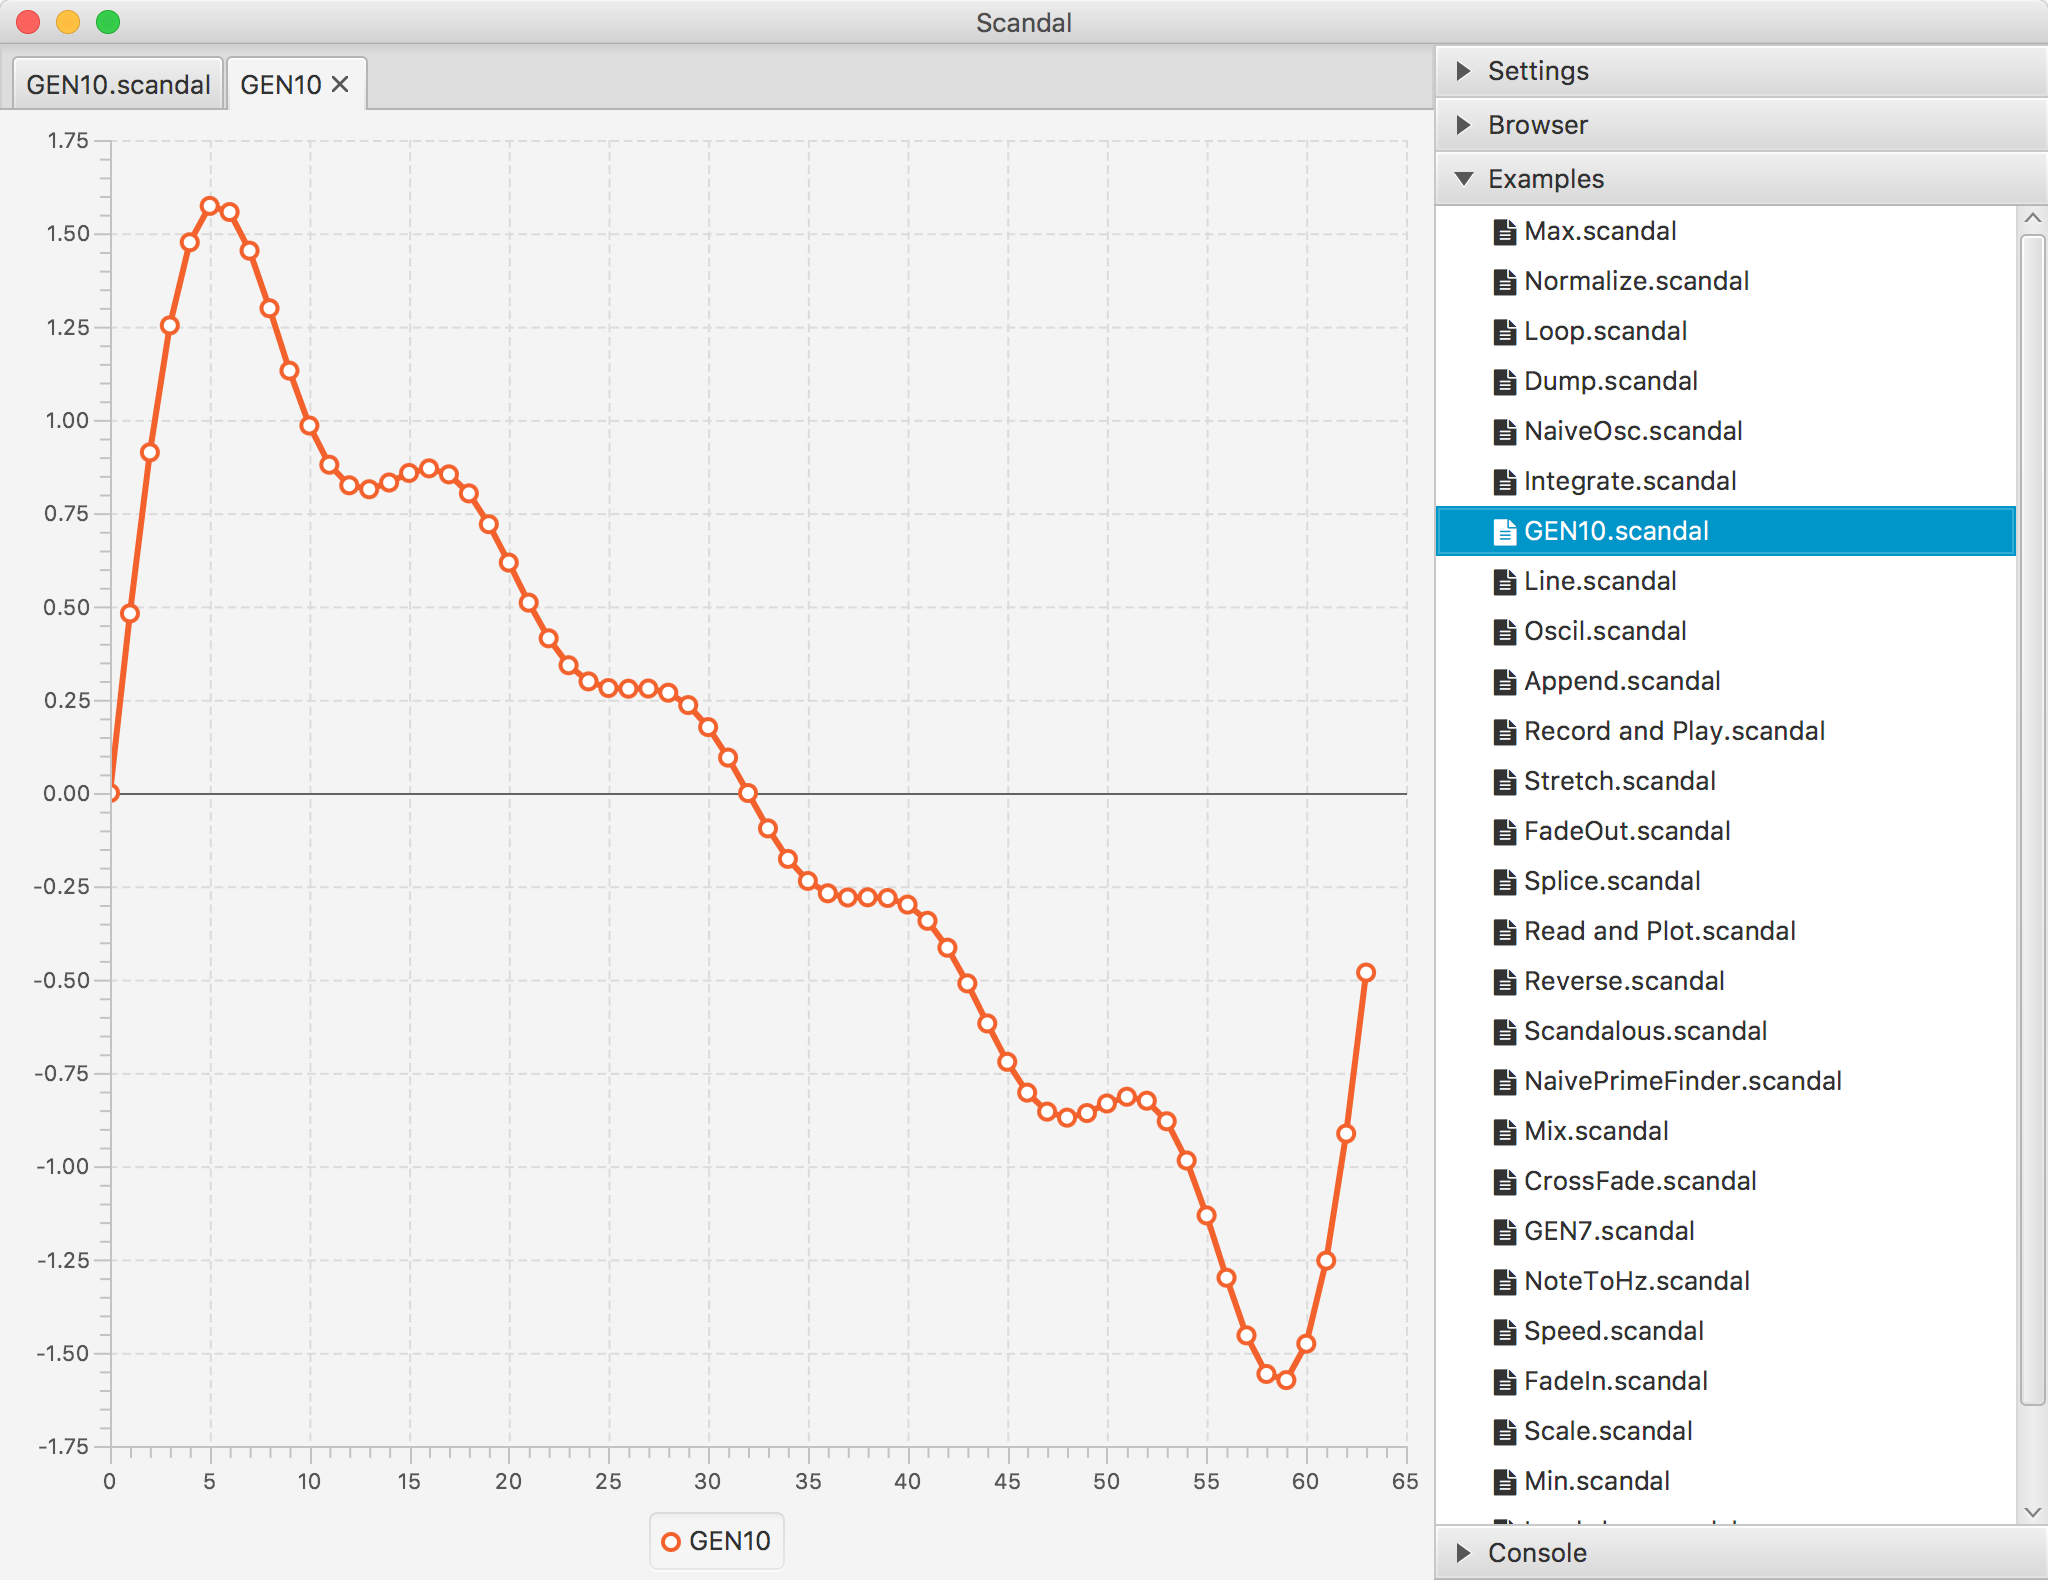
\includegraphics[width=4.5in]{img/plot}
	\caption[Plotting an array in \emph{Scandal}.]{Plotting an array in \emph{Scandal}.}
\end{figure}

\newpage Play statements take an array of audio samples and an integer number of channels, hence extend \il{Statement} by adding to it a second expression property. Parsing is done exactly the same way it is for plot statements, only there is one less expression to parse. The last type of framework statement in the language deals with saving a \emph{.wav} file to disk. Write statements take three arguments, namely the array containing audio samples, a string containing a path in the file system, and an integer number of channels. Parsing follows the exact same pattern found in other framework statements.

\section{Subclasses of \il{Expression}}

The abstract class \il{Expression} has a very diverse family of subclasses, and extends \il{Node} by adding to it three static methods. These methods are type converters and will be discussed in the context of lambda expressions. \il{Expression} neither implements \il{decorate} or \il{generate}, nor adds any properties to \il{Node}, hence remaining a fairly general type of node. Given their diversity, and the fact that often expressions come as binary sub-trees of the AST, expressions are by very far the most difficult construct in the language to parse. The \il{expression} routine in the parser, given below in Listing \ref{alg:expr}, works by always looking for operator tokens, then forming a binary expression whenever applicable. Hence, even when a simple literal expression is given, parsing thereof goes through several steps before being delegated to the specific parsing routine for that particular type of literal. In particular, parsing expressions begins by assuming the expression given is a binary expression containing a lowest-precedence comparison operator. Binary expressions extend \il{Expression} by overriding its abstract methods and adding to it three properties, namely a left-hand side expression, an operation token, and a right-hand expression. Below are the abstract syntax rules for expressions, wherein the rules for operators are the same as the concrete rules, except that instead of strings of characters, the abstract counterparts are given by instances of \il{Token}.

\begin{itemize}
	\item Expression := BinaryExpression $|$ DerivedExpression $|$ LiteralExpression
	\item Expression := ArrayExpression $|$ FrameworkExpression $|$ LambdaExpression
	\item BinaryExpression := Expression\_0 Operator Expression\_1
	\item Operator := ComparisonOperator $|$ SummandOperator $|$ FactorOperator
\end{itemize}

\begin{lstlisting}[language=Java,caption={Parsing Expressions.},label={alg:expr}]
public Expression expression() throws Exception {
	Token firstToken = token;
	Expression e0;
	Token operator;
	Expression e1;
	e0 = comparison();
	while (token.isComparison()) {
		operator = consume();
		e1 = comparison();
		e0 = new BinaryExpression(firstToken, e0, operator, e1);
	}
	return e0;
}
\end{lstlisting}

\begin{enumerate}
	\addtocounter{enumi}{2}
	\item Lines 3 to 5 declare two expressions, one for each node of the assumed binary sub-tree of the AST whose root is returned in line 12, and an operator token.
	\addtocounter{enumi}{2}
	\item Line 6 asks the \il{comparison} routine to provide the left-hand side expression, and line 7 tests in a while-loop to see whether the next token is a comparison operator. If so, the operator is stored and consumed in line 8, line 9 asks \il{comparison} for the right-hand side expression, and line 10 creates an instance of \il{BinaryExpression} with the two expressions. While the next token is still a comparison operator, the while-loop in line 7 keeps asking \il{comparison} for a new right-hand side, then substituting the current instance of \il{BinaryExpression} with another in which the left-hand side is the entire binary expression parsed last, and the right-hand side is the last expression returned from the \il{comparison} method. This method ensures binary expressions always associate equal-precedence operations from left to right.
	\addtocounter{enumi}{5}
	\item Finally, line 12 returns the left-hand side expression, which may or may not be a binary expression.
\end{enumerate}

The \il{comparison} routine does exactly the same \il{expression} does, only checking whether the operator token is at the precedence level of sums. Expressions are instantiated inside \il{comparison} by calling the \il{summand} routine. The \il{summand} routine, in turn, does also exactly the same as \il{expression} and \il{comparison}, only checking whether operator tokens are at the precedence level of products, which is the highest level of precedence among operator tokens in \emph{Scandal}. Expressions are instantiated inside \il{summand} by calling the \il{factor} routine. The latter returns a leaf in the binary tree by looking at the set FIRST(expression), similarly to how declarations and statements are parsed. Some factors, however, require more than one token of look-ahead, namely those that begin with an identifier, with the exception of simple identifier expressions. Inside the \il{factor} routine, whenever a token of kind \texttt{IDENT} is seen, the token next to it needs to be considered so it can be determined whether the factor should be parsed as an indexed array, a lambda application, a lambda composition, or a simple identifier expression. Since two tokens of look-ahead are necessary and enough to parse factors, no other construct in the language requires more than two tokens of look-ahead, constructs are parsed from left to right and leftmost-derived, it follows \emph{Scandal}'s grammar is LL(2).

\subsection{Derived and Literal Expressions}

Parsing derived expressions takes place in the \il{factor} method, as discussed above. For parenthesized expressions, \il{factor} simply looks for a left parenthesis, consumes it, recursively calls the \il{expression} method, then consumes the right parenthesis. Parenthesized expressions are crucial in order to resolve ambiguities, or force the compiler to construct a binary tree for an expression in a certain way. The expression $(1 + 1) / 2$ will be parsed differently than $1 + 1 / 2$, however the AST has no knowledge of parenthesis, it is the way in which binary expression trees are constructed that determines how they are evaluated. Therefore there are no abstract syntax rules for parenthesized expressions, since what they define is not a subtype, but a specific branching of a binary expression tree. Naturally, this tree may be trivial, or identical to a non-parenthesized tree. Such use of the parenthesized expression rule may have a purpose in improving readability of long mathematical expressions. Below are the abstract syntax rules for all derived expressions.

\begin{itemize}
	\item DerivedExpression := UnaryExpression $|$ IdentExpression
	\item UnaryExpression := (Token.\texttt{KW\_MINUS} $|$ Token.\texttt{KW\_NOT}) Expression
	\item IdentExpression := Token.\texttt{IDENT}
\end{itemize}

Unary expressions are parsed by consuming the operator token, then calling \il{expression} in the parser recursively. The \il{UnaryExpression} class extends \il{Node} by adding this referenced expression as a property. The operator is stored as the \il{firstToken} property, which is inherited from the superclass. Identifier expressions extend \il{Node} by adding to it a \il{declaration} property, which is naturally a subclass of \il{Declaration}. Parsing is done in the \il{factor} method, as well. Since the \emph{Scandal} grammar is LL(2), all of the cases in which an expression may begin with an \texttt{IDENT} token are first ruled out before an instance of \il{IdentExpression} is constructed.

All literal expressions extend \il{Expression} by adding no properties to it, since all that is needed is a value for the expression, which is in turn retrieved from the inherited \il{firstToken} property itself. For integers and floats, there is a risk the user will declare a number that is possibly too long. These cases are handled by the scanner at the earliest stage possible, and an informative compilation error is thrown if a bad number is given. In all literal expressions, types are assigned at their onset in the constructor, as type-inference mechanisms are unnecessary.

\subsection{Array Expressions}

For all but the \il{ArrayItemExpression} rule, array expressions are parsed in the \il{factor} method by looking at their first token. In the case of array item expressions, since FOLLOW(\texttt{IDENT}) = $\varepsilon$ $|$ \texttt{LBRACKET} $|$ \texttt{LPAREN} $|$ \texttt{DOT}, one more token of look-ahead is needed, namely a left brace. The other cases are those where a left parenthesis is seen, which correspond to lambda applications, and those in which a dot is seen, corresponding to lambda compositions. After consuming the first token, and possibly the second, parsing follows the same procedure as above, by calling the \il{expression} routine recursively, and abstracting away parenthesis, brackets, commas, and keywords. Below are the abstract rules for array expressions.

\begin{itemize}
	\item ArrayExpression := ArrayLitExpression $|$ ArrayItemExpression
	\item ArrayExpression := ArraySizeExpression $|$ NewArrayExpression
	\item ArrayLitExpression := (Expression)$^+$
	\item ArrayItemExpression := IdentExpression Expression
	\item ArraySizeExpression := Expression
	\item NewArrayExpression := Expression
\end{itemize}

Array literal expressions extend \il{Expression} by adding an \il{ArrayList} of expressions, and naturally overriding its abstract methods. Its type is set to \il{Types.ARRAY} in the constructor, similarly to how literal expressions are handled. Array item expressions extend \il{Expression} with two properties, namely an identifier expression that references the array, and an expression of type integer that stores the index information. Instead of storing an \il{IDENT} token, an \il{IdentExpression} is instantiated while constructing an \il{ArrayItemExpression}. The reason for that is to simplify decoration and code generation by delegating those tasks to the \il{IdentExpression} class, rather than repeating code inside \il{ArrayItemExpression}. Like with literal expressions, the type is always known to be \il{float}, hence set accordingly in the constructor. Array size expressions extend the superclass by including an expression of type \il{array}. Like before, the type is set to \il{int} in the constructor. The last type of array expression deals with creating a new array of zeros with a specified length. An instance of \il{NewArrayExpression} extends \il{Expression} by adding to it a \il{size} expression of integer type. Its type is too set to \il{array} in the constructor.

\subsection{Framework Expressions}

Parsing framework expressions is done in the \il{factor} method by simply looking at the first token at hand and constructing the appropriate subclass of \il{Expression}. Parenthesis, commas, and keywords are naturally all abstracted away. The abstract rules for framework expressions are omitted since they follow the usual pattern of listing all parameters to a framework routine as expressions. The simplest case of a framework expression is that of pi expressions. They extend \il{Expression} only by implementing its abstract methods. Like with literal expressions, its type is set to \il{float} right at construction, and decoration therefore does nothing. Cosine expressions are absolutely fundamental to audio signal processing, and are one of the cases where a pure \il{Scandal} implementation might not be worthwhile. They extend \il{Expression} by adding a \il{phase} property, which is a subclass of \il{Expression} of type \il{float}. Since cosine expressions always have type float in \emph{Scandal}, the type is set in the constructor. Power expressions provide a convenient way to compute exponential expressions, and extend \il{Expression} with two properties, namely \il{base} and \il{exponent}. Floor expressions are identical to cosine expressions, only naturally differing in functionality. Read expressions provide a hook to the audio engine's \il{framework.generators.WaveFile} class, whose main purpose is to parse the contents of a \emph{.wav} file in the file system and return them as an array of floats. \il{ReadExpression} extends the superclass by including two properties, a string \il{path}, and an integer \il{format}, the latter specifying a channel count. The \il{format} property is not overloaded, and accepts only integers. Finally, record expressions connect the DSL with the audio engine's \il{framework.generators.AudioTask} class. They extend \il{Expression} by adding a \il{duration} property, which has type integer but is overloaded to accept floats, as well.

\subsection{Parsing Lambda Expressions}

Parsing lambda literal expressions relies on looking at the first token at hand. Both variants feature a list of parameters separated by arrows, and each parameter is an instance of \il{ParamDeclaration}, hence begins with a type token. Since these are the only two types of expression that begin with a type token, the first token is enough to determine a lambda literal expression. While creating an array of parameter declarations, arrows are abstracted away until no more type tokens are seen. At this point, if a left brace is seen, a lambda block is instantiated and used to construct an instance of \il{LambdaLitBlock}. Otherwise, \il{expression} is called in the parser and the result used to instantiate a \il{LambdaLitExpression}. In fact, \il{LambdaLitBlock} is a subclass of \il{LambdaLitExpression}.

Parsing applications and compositions requires a second token of look-ahead, since both expressions begin with an identifier token. As previously discussed, indexed arrays and identifier expressions are the other two constructs that also begin with an identifier token. What distinguishes all four is the token that follows: indexed arrays are followed by a left bracket, lambda applications are followed by a left parenthesis, lambda compositions are followed by a dot, and identifier expressions are not followed by brackets, parenthesis, or dots. Once a parenthesis is found, the identifier is stored in an instance of \il{IdentExpression}, both parenthesis and all commas are abstracted away, and an instance of \il{LambdaAppExpression} is constructed with the identifier expression and a list of expressions, one for each given argument. If a dot is seen, however, all the subsequent dots are abstracted away while building a list of \il{IdentExpression}. When no more dots are seen, the next token may be a parenthesis or not. If so, an instance of \il{LambdaAppExpression} is used to construct a \il{LambdaCompExpression}, otherwise a null pointer is passed \emph{in lieu} of a \il{LambdaAppExpression} to the constructor of \il{LambdaCompExpression}. Below are the abstract syntax rules for lambda expressions.

\begin{itemize}
	\item LambdaExpression := LambdaLitExpression $|$ LambdaLitBlock
	\item LambdaExpression := LambdaAppExpression $|$ LambdaCompExpression
	\item LambdaLitExpression := ParamDeclaration$^+$ Expression
	\item LambdaLitBlock := ParamDeclaration$^+$ ReturnBlock
	\item ReturnBlock := (AssignmentDeclaration $|$ Statement)$^*$ Expression
	\item LambdaAppExpression := IdentExpression Expression$^+$
	\item LambdaCompExpression := IdentExpression$^+$
	\item LambdaCompExpression := IdentExpression$^+$ LambdaApp
\end{itemize}

\subsubsection{Lambda Literal Expressions}

The \il{LambdaLitExpression} class extends \il{Expression} by including a list of parameter declarations and a return expression, as seen above. In addition to that, it holds an integer property named \il{lambdaSlot}, which is used for naming the lambda in bytecode. Every lambda necessarily has at least one parameter, and necessarily returns a non-void expression. While constructing a lambda literal with expression, its type may be incorrectly inferred by the constructor of \il{Node} to be that of the expression's first token. Hence the expression type is set to \il{Types.LAMBDA} in the constructor of \il{LambdaLitExpression}. The \il{LambdaLitBlock} class is a type of lambda literal expressions in which an entire block of declarations and statements is featured before a return expression is given. Similarly to the superclass, the type of the expression is set to \il{Types.LAMBDA} already in the constructor. Lambda literals with blocks subclass \il{LambdaLitExpression} by adding to it a \il{block} property, that in turn is an instance of \il{ReturnBlock}. Return blocks extend \il{Block} by adding to \il{Block} a return expression property, and this return expression is used in the constructor of a \il{LambdaLitBlock} as an argument to construct the \il{LambdaLitExpression} super class.

\subsubsection{Lambda Applications and Compositions}

An application of a lambda expression in \emph{Scandal} corresponds in the AST to an instance of the \il{LambdaAppExpression} class, which extends \il{Expression} by overriding its abstract methods and including four properties, namely an identifier expression called \il{lambda}, a list of expressions which are the arguments applied to this lambda, an immutable integer property named \il{count}, and a reference to an instance of \il{LambdaLitExpression} called \il{lambdaLit}. While constructing a lambda application expression, the size of the argument list is stored in the \il{count} property, as parameters might be added to this list in the decoration phase. The application type is also set to \il{Types.LAMBDA}, although that too might change if the application is not partial. Lambda compositions correspond to instances of \il{LambdaCompExpression}, which extend \il{Expression} by including two properties, an array of identifier expressions, and a lambda application expression. The latter can be null, as explained in the parsing process. If so, the type of the composition expression is set to \il{Types.LAMBDA} while constructing, otherwise setting a type is deferred until decoration.